%% =====================================================================================
%%  Synthèse (français) de la note « Voting for a consensus with veto rights », v0.1
%% -------------------------------------------------------------------------------------
%%  Compilation : cd summaries/fr/executive && latexmk main.tex
%%  Mise en page : summaries/shared/layout.tex. Chiffres : outputs/tables/key_numbers_fr.tex, écrit par
%%  simulations/python/key_numbers.py -- ne jamais saisir à la main un chiffre calculé par la note.
%%  Garder aligné sur summaries/en/executive/main.tex (même structure, mêmes chiffres).
%% =====================================================================================
\documentclass[10pt,a4paper]{article}
%% ------------------------------------------------------------------------------------------------
%%  Layout of the summaries, shared by every language and every kind of document
%%  (summaries/<lang>/<kind>/<document>.tex, which sets the text and the babel language). Numbers come
%%  from outputs/tables/key_numbers_<lang>.tex. Every document sits two levels below summaries/; the paths
%%  below work from that folder and from the repository root.
%% ------------------------------------------------------------------------------------------------
\usepackage[utf8]{inputenc}
\usepackage[T1]{fontenc}
\usepackage{lmodern}
\usepackage{microtype}
\usepackage{amsmath,amssymb}
\usepackage[a4paper,margin=18mm,top=15mm,bottom=15mm]{geometry}
\usepackage{graphicx}
\usepackage{booktabs,array,tabularx}
\usepackage{xcolor}
\usepackage[most]{tcolorbox}
\usepackage{enumitem}
\usepackage{titlesec}
\usepackage[hidelinks]{hyperref}

\definecolor{accent}{HTML}{2A78D6}      % slot 1 of the figures' palette
\definecolor{accentlight}{HTML}{EAF2FC}
\definecolor{ink}{HTML}{0B0B0B}
\definecolor{muted}{HTML}{52514E}

\setlength{\parindent}{0pt}
\setlength{\parskip}{0.4\baselineskip}
\setlist{itemsep=1pt,topsep=2pt,leftmargin=*}
\pagestyle{plain}

\titleformat{\section}{\normalfont\large\bfseries\color{accent}}{}{0pt}{}
\titlespacing*{\section}{0pt}{8pt}{2pt}

%% A shaded box for the question and the recommendation
\newtcolorbox{keybox}[1]{enhanced, breakable=false, colback=accentlight, colframe=accent,
  boxrule=0.6pt, arc=2pt, left=6pt, right=6pt, top=4pt, bottom=4pt,
  fonttitle=\bfseries, coltitle=white, title={#1}}

%% Title block: \summarytitle{title}{subtitle}{author and date line}
\newcommand{\summarytitle}[3]{%
  {\color{accent}\rule{\linewidth}{1.2pt}}\par\vspace{2pt}
  {\LARGE\bfseries #1\par}\vspace{2pt}
  {\large\color{muted} #2\par}\vspace{2pt}
  {\small\color{muted} #3\par}
  {\color{accent}\rule{\linewidth}{0.6pt}}\par}

\graphicspath{{../../../outputs/figures/}{outputs/figures/}}   % local build, then build from the root

\usepackage[french]{babel}
\frenchsetup{StandardLists=true}          % lists follow the shared layout (enumitem), as in en/
% Generated by simulations/python/key_numbers.py from outputs/tables/*.csv -- do not edit by hand
\newcommand{\KNdeadlockUnanimity}{99{,}6}
\newcommand{\KNdeadlockUnanimityEleven}{86}
\newcommand{\KNcontestedSchulze}{10{,}1}
\newcommand{\KNcontestedQVC}{5{,}9}
\newcommand{\KNworstoffSchulze}{85{,}2}
\newcommand{\KNworstoffQVC}{88{,}4}
\newcommand{\KNworstoffQVCquarter}{92{,}8}
\newcommand{\KNutilitySchulze}{97{,}4}
\newcommand{\KNutilityQVC}{97{,}7}
\newcommand{\KNutilityQVCquarter}{96{,}8}
\newcommand{\KNcontestedQVCquarter}{5{,}9}
\newcommand{\KNdeadlockUnanimityPolarised}{97{,}9}
\newcommand{\KNutilityPlurality}{34}
\newcommand{\KNcondorcetQVC}{94{,}3}
\newcommand{\KNcondorcetQVCquarter}{83{,}2}
\newcommand{\KNcondorcetQVCspatial}{99{,}5}
\newcommand{\KNfallbackQVC}{5{,}9}
\newcommand{\KNfallbackQVCquarter}{27}
\newcommand{\KNclonesPVC}{54}
\newcommand{\KNclonesBorda}{24}
\newcommand{\KNclonesFallback}{36}
\newcommand{\KNclonesPlurality}{98}
\newcommand{\KNmanipSchulzeSpatial}{5}
\newcommand{\KNmanipSchulzePolarised}{7}
\newcommand{\KNmanipQVCSpatial}{11}
\newcommand{\KNmanipQVCPolarised}{27}
\newcommand{\KNmanipQVCquarterSpatial}{52}
\newcommand{\KNmanipQVCquarterPolarised}{57}
\newcommand{\KNcwPolarisedTwelve}{96}
\newcommand{\KNdeadlockUnanimityThree}{43}
\newcommand{\KNclonesSchulze}{0}
\newcommand{\KNclonesQVC}{0}
\newcommand{\KNmanipIRVSpatial}{37}
\newcommand{\KNmanipIRVPolarised}{45}
\newcommand{\KNmanipApprovalSpatial}{85}
\newcommand{\KNmanipApprovalPolarised}{69}
\newcommand{\KNpolCondPlurality}{22{,}4}
\newcommand{\KNpolUtilPlurality}{34{,}4}
\newcommand{\KNpolWorstPlurality}{13{,}3}
\newcommand{\KNpolContestPlurality}{62{,}1}
\newcommand{\KNpolDeadPlurality}{0{,}0}
\newcommand{\KNpolCondBorda}{71{,}2}
\newcommand{\KNpolUtilBorda}{94{,}5}
\newcommand{\KNpolWorstBorda}{79{,}1}
\newcommand{\KNpolContestBorda}{15{,}2}
\newcommand{\KNpolDeadBorda}{0{,}0}
\newcommand{\KNpolCondApproval}{72{,}2}
\newcommand{\KNpolUtilApproval}{95{,}5}
\newcommand{\KNpolWorstApproval}{95{,}0}
\newcommand{\KNpolContestApproval}{5{,}9}
\newcommand{\KNpolDeadApproval}{0{,}0}
\newcommand{\KNpolCondFallback}{53{,}7}
\newcommand{\KNpolUtilFallback}{87{,}7}
\newcommand{\KNpolWorstFallback}{79{,}9}
\newcommand{\KNpolContestFallback}{18{,}6}
\newcommand{\KNpolDeadFallback}{0{,}0}
\newcommand{\KNpolCondUnanimity}{16{,}2}
\newcommand{\KNpolUtilUnanimity}{8{,}5}
\newcommand{\KNpolWorstUnanimity}{30{,}7}
\newcommand{\KNpolContestUnanimity}{57{,}4}
\newcommand{\KNpolDeadUnanimity}{97{,}9}
\newcommand{\KNpolCondSchulze}{100{,}0}
\newcommand{\KNpolUtilSchulze}{97{,}4}
\newcommand{\KNpolWorstSchulze}{85{,}2}
\newcommand{\KNpolContestSchulze}{10{,}1}
\newcommand{\KNpolDeadSchulze}{0{,}0}
\newcommand{\KNpolCondPVC}{90{,}8}
\newcommand{\KNpolUtilPVC}{96{,}2}
\newcommand{\KNpolWorstPVC}{86{,}7}
\newcommand{\KNpolContestPVC}{10{,}2}
\newcommand{\KNpolDeadPVC}{0{,}0}
\newcommand{\KNpolCondQVCquarter}{83{,}2}
\newcommand{\KNpolUtilQVCquarter}{96{,}8}
\newcommand{\KNpolWorstQVCquarter}{92{,}8}
\newcommand{\KNpolContestQVCquarter}{5{,}9}
\newcommand{\KNpolDeadQVCquarter}{0{,}0}
\newcommand{\KNpolCondQVCthird}{94{,}3}
\newcommand{\KNpolUtilQVCthird}{97{,}7}
\newcommand{\KNpolWorstQVCthird}{88{,}4}
\newcommand{\KNpolContestQVCthird}{5{,}9}
\newcommand{\KNpolDeadQVCthird}{0{,}0}


\begin{document}

\summarytitle{Voter pour un consensus avec droit de veto}
{Synthèse de la note d'état de l'art, version 0.1}
{Fabrice Borel-Mathurin \quad$\cdot$\quad 21 octobre 2026 \quad$\cdot$\quad Note complète, code et
données : dépôt \texttt{Vote\_Condorcet}}

\begin{keybox}{La question}
Un groupe doit choisir une option. \textbf{Chacun peut proposer autant d'options qu'il le souhaite},
\textbf{chacun se prononce sur toutes les options} et \textbf{chacun dispose d'un droit de veto}. La
procédure doit aboutir au \textbf{meilleur compromis} et ne doit \textbf{jamais bloquer le groupe}. Que
dit la recherche, et quelle procédure retenir ?
\end{keybox}

\section{L'essentiel}
\begin{enumerate}[label=\textbf{\arabic*.}]
  \item \textbf{Ne pas donner à chacun un veto absolu.} L'unanimité engendre lenteurs, biais en faveur
  du statu quo et obstruction ; avec le statu quo comme option par défaut, elle bloque la décision dans
  \KNdeadlockUnanimityEleven~\% de nos décisions simulées à 11 membres et \KNdeadlockUnanimity~\% à 101.
  \item \textbf{Retenir le \og Condorcet avec quota de blocage\fg{} (QVC), avec un quota d'un tiers.} Un
  seul bulletin ; une option rejetée par au moins un tiers des membres est écartée ; la majorité tranche
  entre les autres.
  \item \textbf{Accepter, et encadrer, son seul coût :} un tiers bloquant peut bloquer de façon
  stratégique. Des vetos nominatifs et motivés, et au plus un tour de révision, le contiennent.
\end{enumerate}

\section{Ce que dit la recherche}
\begin{enumerate}[label=\textbf{\arabic*.}]
  \item \textbf{Il n'existe pas de règle parfaite.} Toute règle de vote peut être manipulée
  (Gibbard--Satterthwaite), et respecter la majorité impose parfois de passer outre une forte minorité :
  concevoir une procédure revient à choisir un arbitrage, qui doit être explicite.
  \item \textbf{L'unanimité est rarement optimale.} Théorie et expériences concordent : elle accroît
  les délais et le pouvoir de ceux qui bloquent ; un vote majoritaire assorti d'un veto \emph{distinct},
  réservé aux issues inacceptables, fait mieux (Bouton et al., 2018 ; Tsebelis, 2002).
  \item \textbf{Le veto doit appartenir à des coalitions, non à des individus,} comme la minorité de
  blocage au Conseil de l'Union européenne ; les instances de consensus telles que l'IETF traitent une
  objection comme un argument à examiner, non comme un blocage.
  \item \textbf{Des propositions libres exigent une règle insensible aux \og clones\fg{}.} Si chacun
  peut ajouter des variantes d'une option, beaucoup de règles récompensent l'inondation de l'ordre du
  jour : trois variantes changent le résultat de la règle de Borda dans jusqu'à \KNclonesBorda~\% de nos
  élections, de la négociation par repli (\emph{fallback bargaining}) dans \KNclonesFallback~\% et du
  noyau de veto proportionnel dans \KNclonesPVC~\%. Les méthodes de Condorcet de type Schulze y sont
  insensibles.
  \item \textbf{Les méthodes de Condorcet donnent les meilleurs résultats lorsque les préférences sont
  structurées,} et un vainqueur de Condorcet (une option préférée par une majorité à chacune des autres)
  existe dans au moins \KNcwPolarisedTwelve~\% de nos électorats simulés, même avec douze options.
\end{enumerate}

\begin{keybox}{Procédure recommandée : QVC($\theta$), avec $\theta = 1/3$}
\begin{enumerate}[label=\textbf{\arabic*.},leftmargin=*]
  \item \textbf{Proposer.} Chacun propose autant d'options qu'il le souhaite. Le statu quo figure sur le
  bulletin comme une option ordinaire, jamais comme option par défaut.
  \item \textbf{Voter une fois.} Chaque membre classe toutes les options (ex aequo admis) et signale
  celles qu'il juge inacceptables ; chaque veto est nominatif et motivé.
  \item \textbf{Filtrer.} Les options frappées de veto par au moins un tiers des membres sont écartées.
  Si toutes le sont, on conserve les options les moins frappées de veto.
  \item \textbf{Décider.} Le vainqueur de Schulze (majorité par duels) parmi les options restantes est
  élu. Les décomptes de vetos et la matrice des duels sont publiés.
  \item \textbf{Réviser, une fois au plus.} Seulement si l'étape 3 a dû recourir au repli : rouvrir
  brièvement les propositions et voter à nouveau ; le second résultat est définitif.
\end{enumerate}
\end{keybox}

\textbf{Ce qu'elle garantit} (démontré dans la note) : elle \textbf{décide toujours}, en un tour (deux
au plus) ; le statu quo ne bénéficie \textbf{d'aucun avantage par défaut} ; le vainqueur est
\textbf{acceptable pour plus des deux tiers} des membres dès qu'une option l'est ; parmi les options
acceptables, \textbf{la majorité décide} ; et \textbf{ajouter des variantes d'une option ne change rien}.

\section{Les résultats chiffrés}
Étude de Monte-Carlo de 21 règles, 2\,000 décisions simulées par configuration, 101 membres, 8 options.
Résultats pour un groupe polarisé (deux blocs de 55~\% et 45~\%), le cas où le compromis compte le plus :

\begin{center}\small
\begin{tabularx}{0.95\linewidth}{X r r r}
\toprule
 & \textbf{Majorité seule} & \textbf{QVC, $\theta = 1/3$} & \textbf{QVC, $\theta = 1/4$} \\
 & (Schulze) & (recommandé) & (plus consensuel) \\
\midrule
Issue rejetée par au moins un tiers des membres & \KNcontestedSchulze~\% & \KNcontestedQVC~\% & \KNcontestedQVCquarter~\% \\
Satisfaction des membres les moins satisfaits (0--100) & \KNworstoffSchulze & \KNworstoffQVC & \KNworstoffQVCquarter \\
Satisfaction totale (0--100) & \KNutilitySchulze & \KNutilityQVC & \KNutilityQVCquarter \\
Option préférée par la majorité élue & 100~\% & \KNcondorcetQVC~\% & \KNcondorcetQVCquarter~\% \\
Manipulable par 10~\% des membres & \KNmanipSchulzePolarised~\% & \KNmanipQVCPolarised~\% & \KNmanipQVCquarterPolarised~\% \\
\bottomrule
\end{tabularx}
\end{center}
{\footnotesize\color{muted} Satisfaction : 0 pour une option moyenne, 100 pour la meilleure ; le membre
le moins satisfait est celui du 10\textsuperscript{e} centile. \og Rejetée par un tiers\fg{} :
\KNcontestedQVC~\% est le minimum atteignable par toute règle, soit la part des décisions où chaque option
est rejetée par un tiers. Unanimité avec le statu quo par défaut, dans la même configuration : blocage
dans \KNdeadlockUnanimityPolarised~\% des décisions.\par}

\textbf{Lecture.} Avec un tiers bloquant, \textbf{les issues contestées sont presque divisées par deux}
et les membres les moins satisfaits s'en sortent mieux, \textbf{sans perte de satisfaction totale} ; le
choix de la majorité n'est écarté que lorsqu'un tiers des membres le rejette. Abaisser le quota à un
quart protège davantage les minorités, mais double l'exposition au blocage stratégique.

\begin{center}
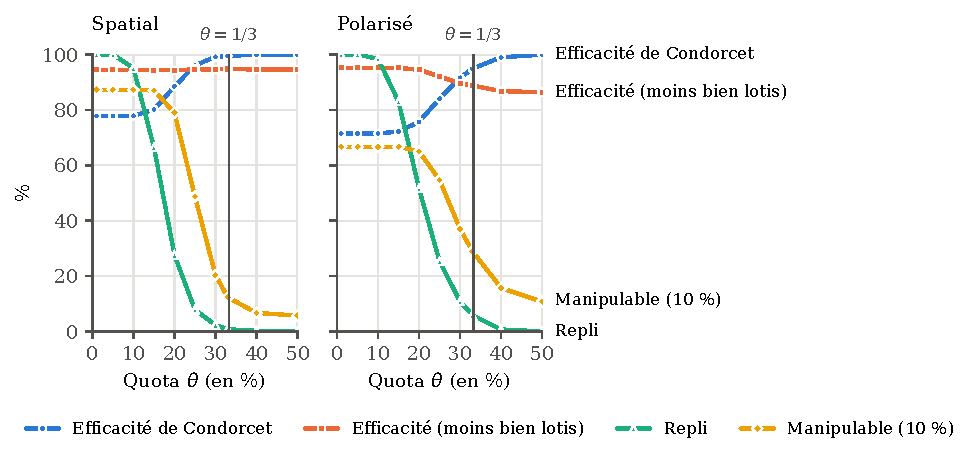
\includegraphics[width=0.8\linewidth]{fig_theta_fr}\\[-2pt]
{\footnotesize\color{muted} Ce que le quota $\theta$ apporte et ce qu'il coûte. En dessous de 20~\%,
presque toutes les options sont frappées de veto et la procédure se replie sur la moins rejetée ;
au-delà de 40~\%, les vetos ne jouent presque plus. Un tiers équilibre les deux.\par}
\end{center}

\section{Le coût, et comment le contenir}
Toute minorité de blocage peut aussi bloquer une option qu'elle juge acceptable, pour favoriser la
sienne : aucune règle de dépouillement ne peut l'empêcher (Greenberg, 1979). Dans nos simulations, une
coalition de 10~\% des membres peut manipuler \KNmanipQVCSpatial{} à \KNmanipQVCPolarised~\% des
décisions avec QVC($1/3$), contre \KNmanipSchulzeSpatial{} à \KNmanipSchulzePolarised~\% avec la seule
règle majoritaire. Garde-fous : \textbf{des vetos publics et motivés} (le président de séance peut écarter
un veto non motivé) ; \textbf{un quota jamais inférieur au quart} ; \textbf{un tour de révision au plus} ;
dans les instances qui décident souvent, \textbf{un budget de vetos réparti sur l'ensemble des
décisions}, jamais au sein d'une même décision.

\section{Décisions à prendre par l'organisation}
\begin{itemize}
  \item \textbf{Quota :} un tiers par défaut (avec 10 membres, 4 vetos écartent une option) ; un quart
  pour une culture plus consensuelle.
  \item \textbf{Statu quo :} une option ordinaire par défaut ; pour les décisions irréversibles, exiger
  que le vainqueur le batte selon un rapport fixé (par exemple 2 contre 1), comme le fait Debian.
  \item \textbf{Tour de révision :} activé ou non, et sa durée.
\end{itemize}

{\footnotesize\color{muted}\textbf{Limites.} Les simulations portent sur des électorats stylisés ; les
références ont été vérifiées sur les pages des éditeurs, non sur les textes intégraux. Prochaine étape :
tester la procédure sur de vrais bulletins classés (par exemple les votes publiés de Debian).\par}

\end{document}
